%!TeX root=../tese.tex
\chapter{Resultados clássicos}
\label{cap:classicos}

Nesse capítulo, iremos apresentar alguns resultados clássicos sobre grafos livres de triângulos, bem como enunciar a Conjectura que iremos explorar nos demais capítulos desse trabalho.

\section{Estabilidade em grafos livres de triângulos}

Historicamente, um dos primeiros resultados provados no que futuramente viria a ser conhecido como Teoria Extremal dos Grafos é o Teorema de Mantel.

\begin{theorem}[\cite{mantel1907problem}]~\label{thm:mantel}
  Seja $G$ um grafo livre de triângulos com $n$ vértices.
  Então $e(G) \leq \lfloor n^2/4 \rfloor$.
  Além disso, $e(G)=\lfloor n^2/4 \rfloor$ se, e somente se, $G$ é um grafo bipartido completo em que uma das classes tem tamanho $\lfloor n/2 \rfloor$, e a outra tem tamanho $\lceil n/2 \rceil$.
\end{theorem}
Omitimos a prova do Teorema~\ref{thm:mantel} nessa seção.
No Capítulo~\ref{cap:flag-algebras}, apresentaremos uma prova do Teorema~\ref{thm:mantel} usando ferramentas modernas de Teoria Extremal dos Grafos, que servirá de motivação para o restante do Capítulo~\ref{cap:flag-algebras}.
De toda forma, provas elementares do Teorema~\ref{thm:mantel} podem ser encontradas nas referências básicas da área (ver~\cite{livrocombinatoria}).

O Teorema~\ref{thm:mantel} impõe uma restrição bastante forte sobre grafos livres de triângulos muito \emph{densos} (isto é, grafos com muitas arestas).
Ao mesmo tempo que se permite que um grafo livre de triângulos tenha aproximadamente metade das arestas ``disponíveis'' (uma vez que o número máximo de arestas possíveis em um grafo com $n$ vértices é $\binom{n}{2} \approx 2 \cdot \frac{n^2}{4}$), ele impõe uma forte restrição estrutural sobre tais grafos: para cada $n$, existe essencialmente um \emph{único} grafo livre de triângulos com $n$ vértices e $e(G) = \lfloor n^2/4 \rfloor$.

De forma paralela, podemos pensar em formas gerais de descrever grafos livres de triângulos e maximizar o número de arestas disponíveis.
Por exemplos, os grafos bipartidos são claramente livres de triângulos, pois para quaisquer três vértices do grafo há dois na mesma parte pelo Princípio da Casa dos Pombos, e tais dois vértices não fazem parte de um triângulo pois não são vizinhos.
Além disso, um grafo bipartido $G$ com bipartição $V(G) = A \cup B$ possui, no máximo $|A||B| = |A|(n-|A|) \leq \lfloor n^2/4 \rfloor$ arestas, com igualdade se e somente se $\{|A|,|B|\}=\{\lfloor n/2 \rfloor, \lceil n/2 \rceil\}$.

Em conclusão, observa-se uma relação muito próxima entre a família de grafos livres de triângulos densos e a família de grafos bipartidos, e o Teorema~\ref{thm:mantel} sugere uma aproximação entre as duas famílias quando a densidade do grafo aumenta.
É portanto natural se perguntar se se estende tal analogia entre as duas classes de grafos: \emph{quão ``distante'' pode estar um grafo livre de triângulos de ser bipartido?}
A noção de distância que iremos utilizar é formalizada pela definição a seguir:

\begin{definition}
  Seja $G$ um grafo.
  Definimos $D(G)$ como o menor tamanho de um conjunto de arestas $F \subseteq G$ tal que $G-F \coloneqq (V(G),E(G) \setminus F)$ é bipartido.
\end{definition}

O próximo teorema é um teorema clássico de \emph{estabilidade}, e dá uma resposta inicial para a nossa pergunta.

\begin{theorem}[\cite{simonovits1968stability}] \label{thm:estabilidade}
  Seja $m \geq 0$ um inteiro e seja $G$ um grafo livre de triângulos com $n$ vértices e $\frac{n^2}{4}-m$ arestas.
  Então $D(G) \leq m$.
\end{theorem}

O Teorema~\ref{thm:estabilidade} pode ser interpretado como um resultado estrutural: quanto mais arestas queremos que um grafo livre de triângulos tenha, mais restrita será a estrutura desse grafo.
Esse paradigma voltará no Capítulo~\ref{cap:grau-limitado}, quando em vez de usarmos o número de arestas para parametrizar a densidade de grafos livres de triângulos, usarmos o seu grau mínimo.

A prova do Teorema~\ref{thm:estabilidade} pode ser encontrada no Capítulo 3 de~\cite{livrocombinatoria}, mas os métodos utilizados na prova do Teorema de Mantel que apresentaremos no Capítulo~\ref{cap:flag-algebras} permitem obter resultados similares de estabilidade.
Mais resultados relacionados a estabilidade em grafos podem ser vistos em~\cite{furedi2015stability,taisa2021cuts,sudakov2007k4}.

Para grafos com apenas poucas arestas a menos que $n^2/4$, o Teorema~\ref{thm:estabilidade} fornece uma cota superior satisfatória para $D(G)$.
Em 1975, Erd{\H o}s propôs a seguinte conjectura para uma cota \emph{incondicional} sobre $D(G)$, no sentido que ela não depende do número de arestas de $G$.

\begin{conjecture} [\cite{erdos1975problems}] \label{conj:make-bipartite}
  Seja $G$ um grafo livre de triângulos com $n$ vértices.
  Então \[D(G) \leq \frac{n^2}{25}.\]
\end{conjecture}

A Conjectura~\ref{conj:make-bipartite} permanece em aberto no caso geral.

Observe que o Teorema \ref{thm:estabilidade} prova a Conjetura~\ref{conj:make-bipartite} com pelo menos $21n^2/100$ arestas.
Além disso, se verdadeira, a cota $n^2/25$ é ótima, pois o grafo $G$ que é um blow-up balanceado de $C_5$ com $n=5m$ vértices satisfaz $D(G) = m^2 = n^2/25$.

\begin{figure}[htbp]
\centering
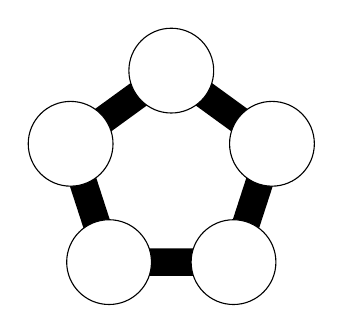
\begin{tikzpicture}[scale=1.5,x=0.75pt,y=0.75pt,yscale=-1,xscale=1]
%uncomment if require: \path (0,300); %set diagram left start at 0, and has height of 300

%Shape: Regular Polygon [id:dp431228592973964] 
\draw  [color={rgb, 255:red, 0; green, 0; blue, 0 }  ,draw opacity=1 ][line width=10]  (128.72,89.33) -- (161.06,112.82) -- (148.7,150.83) -- (108.74,150.83) -- (96.38,112.82) -- cycle ;
%Shape: Circle [id:dp30642581066378904] 
\draw  [fill={rgb, 255:red, 255; green, 255; blue, 255 }  ,fill opacity=1 ] (82.77,112.82) .. controls (82.77,105.3) and (88.86,99.21) .. (96.38,99.21) .. controls (103.9,99.21) and (110,105.3) .. (110,112.82) .. controls (110,120.34) and (103.9,126.44) .. (96.38,126.44) .. controls (88.86,126.44) and (82.77,120.34) .. (82.77,112.82) -- cycle ;
%Shape: Circle [id:dp047385789315699256] 
\draw  [fill={rgb, 255:red, 255; green, 255; blue, 255 }  ,fill opacity=1 ] (115.1,89.33) .. controls (115.1,81.81) and (121.2,75.71) .. (128.72,75.71) .. controls (136.24,75.71) and (142.34,81.81) .. (142.34,89.33) .. controls (142.34,96.85) and (136.24,102.94) .. (128.72,102.94) .. controls (121.2,102.94) and (115.1,96.85) .. (115.1,89.33) -- cycle ;
%Shape: Circle [id:dp44176033632730916] 
\draw  [fill={rgb, 255:red, 255; green, 255; blue, 255 }  ,fill opacity=1 ] (147.44,112.82) .. controls (147.44,105.3) and (153.54,99.21) .. (161.06,99.21) .. controls (168.58,99.21) and (174.67,105.3) .. (174.67,112.82) .. controls (174.67,120.34) and (168.58,126.44) .. (161.06,126.44) .. controls (153.54,126.44) and (147.44,120.34) .. (147.44,112.82) -- cycle ;
%Shape: Circle [id:dp2539724003675331] 
\draw  [fill={rgb, 255:red, 255; green, 255; blue, 255 }  ,fill opacity=1 ] (135.09,150.83) .. controls (135.09,143.31) and (141.19,137.22) .. (148.7,137.22) .. controls (156.22,137.22) and (162.32,143.31) .. (162.32,150.83) .. controls (162.32,158.35) and (156.22,164.45) .. (148.7,164.45) .. controls (141.19,164.45) and (135.09,158.35) .. (135.09,150.83) -- cycle ;
%Shape: Circle [id:dp01546028426045376] 
\draw  [fill={rgb, 255:red, 255; green, 255; blue, 255 }  ,fill opacity=1 ] (95.12,150.83) .. controls (95.12,143.31) and (101.22,137.22) .. (108.74,137.22) .. controls (116.26,137.22) and (122.35,143.31) .. (122.35,150.83) .. controls (122.35,158.35) and (116.26,164.45) .. (108.74,164.45) .. controls (101.22,164.45) and (95.12,158.35) .. (95.12,150.83) -- cycle ;
\end{tikzpicture}
\caption{}
\label{fig:c5-blowup}
\end{figure}

%Os $5m$ vértices estão particionados nas classes representadas, cada uma de tamanho $m$.
%Uma ``aresta grossa'' na figura representa que todas as arestas entre vértices das duas classes unidas pertencem ao grafo.
É fácil ver que o $G$ é livre de triângulos e $D(G) \leq m^2$, pois ao remover todas as arestas entre um par de classes da partição o subgrafo restante se torna bipartido.
Por outro lado, segue do Teorema~\ref{thm:simetrizacao} que existe uma coleção de ``arestas grossas'' de $G$ cuja remoção deixa $G$ bipartido e o total de arestas removidas é igual a $D(G)$, ou seja, $D(G) \geq m^2$.

%O grafo da Figura~\ref{fig:c5-blowup} pode ser visto como um grafo obtido a partir de uma ``explosão'' dos vértices de $C_5$.
%Tal explosão é chamada de \emph{blow-up} de um grafo:

%\begin{definition}
%  Seja $G$ um grafo.
%  Dizemos que um grafo $H$ é um \emph{blow-up} de $G$ se cada vértice de $G$ é substituído por um conjunto independente de vértices.
%  Formalmente, para cada $v \in V(G)$, existe $S_v \subseteq V(H)$ e:
%  \begin{itemize}
%    \item $\{S_v : v \in V(G)\}$ é uma partição de $V(H)$;
%    \item Para cada $xy \in E(H)$ e $u,v \in V(G)$, vale que $(x,y) \in S_u \times S_v \iff uv \in E(G)$. 
%  \end{itemize}
%\end{definition}
%
%Um blow-up é chamado de \emph{balanceado} se todos os conjuntos $S_v$ têm o mesmo tamanho.
%Observe que um grafo $G$ é homomórfico a um grafo $H$ se, e somente se, $G$ é um subgrafo de um blow-up adequado de $H$.

Os blow-ups serão amplamente utilizados nos capítulos a seguir no estudo da Conjectura~\ref{conj:make-bipartite}.
Eles são grafos úteis porque se um grafo (grande) $G$ é um blow-up de um grafo (pequeno) $H$, então uma série de comportamentos em $G$ ``imitam os comportamentos análogos'' em $G$, e portanto podemos descrever certas propriedades de $G$ usando os parâmetros de $H$, que são menos.
O Teorema~\ref{thm:simetrizacao} deixará essa utilidade evidente, mas antes de prová-lo precisamos definir de forma precisa a ``analogia'' entre $G$ e $H$.

\begin{definition}
  Seja $G$ um blow-up de $H$ e seja $V(G) = \{S_v : v \in V(H)\}$ uma partição de $H$ que satisfaz a definição de blow-up.
  Dizemos que $F_G \subseteq E(G)$ é \emph{canônico} se existe $F_H \subseteq H$ tal que
  \[ F_G = \bigcup_{uv \in F_H} E(G[S_u \cup S_v]). \]
  Em outras palavras, um conjunto canônico de arestas é tal que, entre cada par de classes de $V(G)$, ou adicionamos todas as arestas entre essas classes para o conjunto, ou não adicionamos nenhuma dessas arestas.
\end{definition}

É prudente observar que a definição de um conjunto canônico depende da escolha da partição de $V(G)$ (que não necessariamente é única).
Em geral, essa escolha será clara do contexto.

\begin{theorem}[\cite{erdos1992many}]\label{thm:simetrizacao}
  Seja $H$ um grafo livre de triângulos e seja $G$ um blow-up de $H$.
  Então existe $F \subseteq E(G)$ canônico tal que $|F|=D(G)$ e $G-F$ é bipartido.
\end{theorem}
\begin{proof}
  A prova usa um procedimento conhecido como \emph{simetrização de Zykov}.
  Em linhas gerais, a ideia é que se $u$ e $v$ estão na mesma parte e $d_Z(u) \geq d_Z(v)$ para um certo subgrafo bipartido $Z$ de $G$, então trocar a vizinhança de $v$ em $Z$ para $N_Z(u)$ não muda a propriedade de $Z$ ser bipartido, não diminui o número de arestas de $Z$ e o torna mais ``simétrico'' de forma que esse procedimento pode ser realizado apenas finitamente.

  Seja $Z$ um subgrafo gerador de $G$ tal que $Z$ é bipartido e $e(G)-e(Z_0)=D(G)$.
  Vamos definir $Z_0 \coloneqq Z$ e modificar $Z_0$ sem diminuir seu número de arestas e garantindo que a propriedade da bipartição é mantida.
  Para isso, ordene as classes do blow-up $H$ como $V(G) = \{S_1,S_2,\dots,S_n\}$ e aplique a seguinte operação sequencialmente para cada $i \in [n]$:
  \begin{itemize}
    \item Tome $x \in S_i$ com grau máximo em $Z_{i-1}$;
    \item Para cada $y \in S_i \setminus \{x\}$, forme $Z_i$ substituindo a vizinhança de $y$ em $Z_{i-1}$ por $N_Z(x)$.
  \end{itemize}
  Perceba que pela maximalidade de $N_{Z_{i-1}}(x)$, o número de arestas do grafo não diminui a cada substituição de vizinhanças.
  Além disso, a propriedade da bipartição é mantida: depois de substituir a vizinhança de $y$, coloque $y$ na mesma classe da bipartição em que está $x$.

  Em $Z_n$, todos os pares $x,y$ pertencendo à mesma parte de $\{S_1,S_2,\dots,S_n\}$ terão a mesma vizinhança.
  Além disso, se $xy \in E(Z_n)$ com $x \in S_u$ e $y \in S_v$, então $x'y \in E(Z_n)$ para cada $x' \in S_u$ (pela simetria em $S_u$) e $xy' \in E(Z_n)$ para cada $y' \in S_v$ (pela simetria em $S_v$).
  Dessa forma, $F \coloneqq E(H) \setminus E(Z')$ é um conjunto canônico de arestas de cardinalidade $e(H)-e(Z_n) \leq e(H)-e(Z_0) = D(H)$.
  Pela definição de $D(H)$, segue que a igualdade vale, e $|F| = D(H)$, como desejado.
\end{proof}

\section{Avanços parciais na Conjectura~\ref{conj:make-bipartite}}

Ao longo dos anos, as tentativas de resolução da Conjectura~\ref{conj:make-bipartite} levaram a importantes resultados parciais.
Existem duas formas principais de produzir resultados parciais na direção da Conjectura~\ref{conj:make-bipartite}: restringindo a família de grafos $G$ (por exemplo, a um número máximo/mínimo de arestas) ou provando cotas mais fracas para $D(G)$.
O seguinte teorema foi usado para obter resultados parciais nas duas condições (Corolário~\ref{cor:n2/18} e Teorema~\ref{thm:n2/5}).

\begin{theorem}[\cite{erdos1988make}] \label{thm:EFPS-bounds}
  Seja $G$ um grafo livre de triângulos com $n$ vértices e $m$ arestas.
  Então \[ D(G) \leq \min\left\{m-\frac{4m^2}{n^2}, \frac{m}{2} - \frac{2m(2m^2-n^3)}{n^2(n^2-2m)}\right\}. \]
\end{theorem}
\begin{proof}
  A prova da desigualdade $D(G) \leq m-\frac{4m^2}{n^2}$, bem como a ideia principal por trás da contagem que leva à cota $D(G) \leq \frac{m}{2} - \frac{2m(2m^2-n^3)}{n^2(n^2-2m)}$, serão generalizadas na Seção~\ref{sub:cortes_locais}.
  Por ora, provaremos apenas $D(G) \leq m-\frac{4m^2}{n^2}$, utilizando um argumento simples de contagem que importantes propriedades de grafos livres de triângulos que usaremos para localizar subgrafos bipartidos grandes.

  Para cada vértice $v \in V(G)$, defina o conjunto $F_v \coloneqq V(G) \setminus N_G(v)$ (os não vizinhos de $v$, incluindo o próprio $v$).
  Note que $D(G) \leq |F_v|$ para qualquer vértice $v$, pois a bipartição $\{N_G(v), V(G) \setminus N_G(v)\}$ possui exatamente $|F_v|$ arestas dentro da segunda parte, e a primeira é independente.
  Assim, temos que
  \begin{equation}\label{eq:bound-with-Fs}
     D(G) \leq \min_{v \in V(G)} |F_v| \leq \frac{1}{n} \sum_{v \in V(G)} |F_v|.
  \end{equation} 
  Observe que se $xy \in F_v$, então $v \in V(G) \setminus (N_G(x) \cup N_G(y))$, logo cada aresta $xy \in E(G)$ pertence a no máximo $n-d_G(x)-d_G(y)$ conjuntos $F_v$.
  Aplicando essa cota em (\ref{eq:bound-with-Fs}), temos
  \begin{align*}
    D(G) &\leq \frac{1}{n} \sum_{v \in V(G)} |F_v| \\
      &\leq \frac{1}{n} \sum_{xy \in E(G)} (n-d_G(x)-d_G(y)) \\
      &= m - \frac{1}{n} \sum_{x \in V(G)} d_G(x)^2 \\
      &\leq m-\left(\frac{\sum_{x \in V(G)} d_G(x)}{n}\right)^2 \\
      &=m-\frac{4m^2}{n^2}.
  \end{align*}

\end{proof}

\begin{corollary}[\cite{erdos1988make}] \label{cor:n2/18}
  Se $G$ é um grafo livre de triângulos com $n$ vértices, então $D(G) \leq n^2/18$.
\end{corollary}
De fato, o resultado de~\cite{erdos1988make} é mais justo: analisando os casos próximos à igualdade, é possível provar que existe $\varepsilon>0$ tal que $D(G) \leq (1/18-\varepsilon)n^2$.
A análise é direta, mas não trivial.%, e não segue apenas das cotas do Teorema~\ref{thm:EFPS-bounds}.

\begin{theorem}[\cite{erdos1988make}] \label{thm:n2/5}
  Para todo $n$ inteiro positivo, a Conjectura \ref{conj:make-bipartite}
  é verdadeira para grafos com $n$ vértices e pelo menos $n^2/5$ arestas.
\end{theorem}

O Teorema~\ref{thm:n2/5} dá uma melhora aparentemente pequena sobre a cota inferior de $e(G)$ para a qual a Conjectura~\ref{conj:make-bipartite} é válida: de $e(G) \geq 0.21n^2$ usando o Teorema~\ref{thm:estabilidade} para $e(G) \geq 0.20n^2$ usando o Teorema~\ref{thm:n2/5}.
Porém, acontece que $e(G) \geq n^2/5$ não é apenas uma melhora pequena, mas também um ``limiar estrutural'' para grafos livres de triângulos longe de serem bipartidos.

%Por um lado, o exemplo da Figura~\ref{fig:c5-blowup} é o único exemplo extremal conhecido, e o próximo teorema mostra que os blow-ups de $C_5$ são os exemplos que maximizam $D(G)$ se $e(G) \geq n^2/5$ é dado.
\begin{theorem}[\cite{erdos1992many}]\label{thm:dG-dH-blowup-C5}
  Seja $G$ um grafo livre de triângulos com $n$ vértices e pelo menos $n^2/5$ arestas.
  Então existe um grafo $H^*$ também com $n$ vértices tal que $H^*$ é um blow-up de $C_5$ e, além disso,
  $e(G) \leq e(H^*)$ e $D(G) \leq D(H^*)$.
\end{theorem}

É fácil ver que $\max_{e(H^*) \geq m}D(H^*)$ (máximo tomado sobre os blow-ups $H^*$ de $C_5$) é decrescente em $m$ para $m \geq n^2/5$, o que dá uma cota melhor que $n^2/5$ para $e(G) \geq n^2/5$, condicionando no valor de $e(G)$.
Do resultado do Teorema~\ref{thm:dG-dH-blowup-C5} também segue que o único exemplo extremal para a Conjectura~\ref{conj:make-bipartite} quando $e(G) \geq n^2/5$ são os blow-ups balanceados de $C_5$.
Não é conhecido nenhum outro exemplo extremal.

Omitiremos a prova completa do Teorema~\ref{thm:dG-dH-blowup-C5} e daremos apenas um brevíssimo esboço.
As técnicas utilizadas não serão replicadas em outras partes desse trabalhos e requerem muitos cuidados com as contas.
Os detalhes podem ser encontrados em~\cite{erdos1992many}.

\begin{proof}[Esboço da demonstração do Teorema~\ref{thm:dG-dH-blowup-C5}]
  Definimos os dois conjuntos que formam a ``quase bipartição'' do grafo de forma algorítmica.
  Primeiro, escolhemos uma aresta $xy$ com $d_G(x)+d_G(y)$ máximo e os conjuntos da bipartição $A_1 \coloneqq N_G(x)$ e $A_2 \coloneqq N_G(y)$.
  Como $G$ é livre de triângulos, cada vértice de $G$ pertence a no máximo uma dessa partes.
  Além disso, se $e(G) \geq n^2/5$, então é fácil ver que o número de vértices que ainda não tem lado definido é no máximo $n^2/5$.
  Iterativamente, adiciona-se sequencialmente cada um dos vértices restantes a $A_1$ ou $A_2$ de forma a minimizar o número de arestas ``monocromáticas'' (isso é, entre vértices da mesma parte) a cada passo.
  Esses novos vértices formam conjuntos $C_1$ e $C_2$, respectivamente.

  A partir desse ponto, a prova segue dois caminhos:
  \begin{itemize}
    \item Se existe algum vértice $x_0 \in C_1 \cup C_2$ (suponha sem perda de generalidade que $x_0 \in C_1$) que tem pelo menos $|C_1 \cup C_2|$ vizinhos em $C_1$, então é possível definir os tamanhos das classe de $H^*$ usando os conjuntos que já temos e as vizinhanças de $x_0$ em $C_1$ e $C_2$.
    As definições precisas dos tamanhos das classes são omitidas aqui.
    \item Se não existe tal vértice, então usando conjuntos de arestas duas a duas disjuntas (de tamanho cotado superiormente) em $A_1 \cup C_1$ e em $A_2 \cup C_2$, é possível descrever os tamanhos das classes de $H^*$ de forma similar.
    Os detalhes numéricos desse caso também são omitidos aqui.
  \end{itemize}
\end{proof}


Por fim, apresentamos uma conjectura relacionada à Conjectura~\ref{conj:make-bipartite}:
\begin{conjecture} [\cite{erdos1975problems}] \label{conj:metadinha}
  Seja $G$ um grafo livre de triângulos com $n$ vértices.
  Então existe $X \subseteq V(G)$ com $X = \lfloor n/2 \rfloor$ tal que $e(G[X]) \leq n^2/50$.
\end{conjecture}
Posteriormente, Erd\H os ofereceu um prêmio monetário de \$ 250 para uma prova ou contraexemplo da Conjectura~\ref{conj:metadinha}~\cite{erdHos1997some}.

Resultados similares ao Teorema~\ref{thm:n2/5} foram verificados para a Conjectura~\ref{conj:metadinha}~\cite{keevash2006sparsehalves}.
Além disso, Krivelevich observou (ver~\cite{krivelevich1995edge}) que a Conjectura~\ref{conj:metadinha} implica a Conjetura~\ref{conj:make-bipartite} para grafos regulares: se $X$ é o conjunto fornecido pela resposta à Conjectura~\ref{conj:metadinha} para $G$, então $e(G[X])=e(G[V(G) \setminus X])$ pela regularidade de $G$, e segue que o subgrafo bipartido de $G$ induzido pelas partes $X$ e $V(G) \setminus X$ tem, no máximo, $2n^2/50=n^2/25$ arestas a menos que $G$.
